\documentclass[11pt]{article}
\usepackage{amsmath, amsfonts, amssymb}
\usepackage{graphicx}
\usepackage{booktabs}
\usepackage[referable]{threeparttablex}
\usepackage{lipsum}
\usepackage{hyperref}
\usepackage[utf8]{inputenc}
\usepackage[margin = 3cm]{geometry}

\title{Using Taxes to Incentivize Vegetarianism: \\ Evidence from Paella Restaurants}
\author{Víctor Quintas-Martínez}
\begin{document}
\maketitle

\begin{abstract}
\lipsum[1]
\end{abstract}

\section{Introduction}
\lipsum[1-10]

\section{Model}
\subsection{Demand}
We are going to observe data on $T = 1000$ Spanish towns. In each town, there are $N = 500$ consumers deciding between chicken paella and veggie paella, denoted by $j=1$ and $j=2$, respectively. Utility of consumer $i$ in town $t$ if they choose product $j$ is: 
$$u_{ijt} = \delta_j - \alpha p_{jt} + \xi_{jt} + \epsilon_{ij}, \quad j\in\{1,2\}.$$
They can also choose to not consume any paella, which we denote by $j=0$, in which case they receive utility $u_{i0t} = \epsilon_{i0}$. We assume that the $\epsilon_{ij}$ are iid across consumers and products, following an EV type I (or Gumbel) distribution. The $\xi_{jt}$ are town-product specific taste shocks following an iid $\mathcal{N}(0, \sigma)$ distribution, observed by  consumers and firms but not by the econometrician.  

It can be shown (don't worry about the derivations) that, under these distributional assumptions, the expected market share of product $j$ in town $t$ will be:
\begin{align*}
s_{jt}(\mathbf{p}_{t}) & = \frac{\exp(\delta_j - \alpha p_{jt} + \xi_{jt})}{1 + \sum_{k=1}^2 \exp(\delta_k - \alpha p_{kt} + \xi_{kt})}, \quad j\in\{1,2\}, \\ s_{0t}(\mathbf{p}_{t}) & = \frac{1}{1 + \sum_{k=1}^2 \exp(\delta_j - \alpha p_{kt} + \xi_{kt})}. 
\end{align*}

\subsection{Supply}
In each town, there are two restaurants, one that specializes in chicken paellas, and one that specializes in veggie paellas. The prices are set in monopolistic competition, where each restaurant chooses price to maximize profits given the other restaurant's price and the expected demand:
$$\max_{p_{jt}} N \cdot s_{jt}(\mathbf{p}_t) \cdot (p_{jt} - c_{jt}) \quad \text{subj. to } s_{jt}(\mathbf{p}_{t}) = \frac{\exp(\delta_j - \alpha p_{jt} + \xi_{jt})}{1 + \sum_{k=1}^2 \exp(\delta_k - \alpha p_{kt} + \xi_{kt})}, \quad j \in \{1,2\}.$$

Here, $c_{jt}$ is marginal cost. For simplicity, let us supose that $\log c_{jt} \sim \mathcal{N}(0,0.25)$, iid across towns and products, and that this is observed by the econometrician.

\section{Reduced Form}
\lipsum[11-13]

\begin{table}[h]
    \centering
    \begin{threeparttable}
    \caption{Reduced Form Results \label{table}} 
    \vspace{1em}
    \begin{tabular}{lrr}
\toprule
          & \multicolumn{1}{c}{OLS} & \multicolumn{1}{c}{IV} \\ 
\cmidrule(lr){2-2} \cmidrule(lr){3-3} 
          &      \multicolumn{2}{c}{log Relative Share}      \\ 
\cmidrule(lr){2-3} 
          &                     (1) &                    (2) \\ 
\midrule
Product 1 &               -0.622*** &               1.928*** \\ 
          &                 (0.090) &                (0.130) \\ 
Product 2 &               -0.719*** &               1.739*** \\ 
          &                 (0.087) &                (0.125) \\ 
Price     &                0.141*** &              -0.485*** \\ 
          &                 (0.022) &                (0.032) \\ 
\midrule
$N$       &                   2,000 &                  2,000 \\ 
\bottomrule
\end{tabular}

    \begin{tablenotes}
    \footnotesize \item Robust standard errors in brackets. 
    \item * $p < 0.1$, ** $p < 0.05$, *** $p < 0.01$
    \end{tablenotes}
    \end{threeparttable}  
\end{table}

Table \ref{table} shows the reduced form results.

\lipsum[14-16]

\section{Counterfactuals}
\lipsum[17-20]

\begin{figure}[h]
    \centering
    \caption{Counterfactual Results}
    \label{figure}
    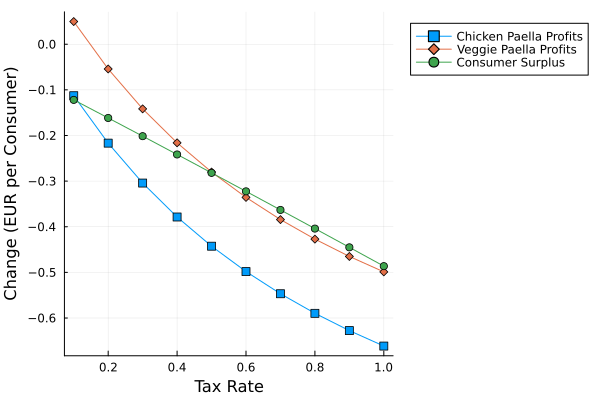
\includegraphics[width = 0.7\textwidth]{\outputpath/figure}
\end{figure}

\lipsum[21-30]

\section{Conclusions}
\lipsum[31-32]

\end{document}